\documentclass[12pt,letterpaper]{article}

\usepackage[spanish,es-tabla,es-nodecimaldot]{babel}
\usepackage{amsmath}
\usepackage[utf8]{inputenc}
\usepackage[T1]{fontenc}
\usepackage{lmodern}
\usepackage{graphicx}
\usepackage{listings}
\usepackage{anysize} 
\usepackage{fancyhdr}
\usepackage{amsmath}
\usepackage{pdfpages}
\usepackage{graphics}
\usepackage{capt-of}
\usepackage{tabularx}
\usepackage[colorlinks=true,plainpages=true,citecolor=blue,linkcolor=blue]{hyperref}

\marginsize{2cm}{2cm}{2cm}{2cm}
\pagestyle{fancy}
\fancyhf{Teoría de la Información}
\fancyhead[L]{\footnotesize UPIITA-IPN} 
\fancyhead[R]{\footnotesize 2TM4} 
\fancyfoot[R]{\footnotesize Entropía del idioma}
\fancyfoot[C]{\thepage}
\fancyfoot[L]{\footnotesize Práctica 1} 
\renewcommand{\footrulewidth}{0.4pt}
\renewcommand{\spanishtablename}{Tabla}
\renewcommand{\labelitemii}{$\star$}
\graphicspath{ {C:/Users/Anselmo-PC/Documents/GitHub/upiita-RedesTelecomunicaciones/MemoriaTecnica/imagenes} }

\begin{document}
\newpage

\newpage
\section{Información del texto}
\begin{itemize}
    \item \textbf{Libro: }Fahrenheit 451.
    \item \textbf{Autor: }Ray bradbury.
    \item \textbf{Publicación: }1953.
    \item \textbf{Lengua original: }Inglés.
    \item \textbf{Cantidad de caracteres inglés: }236676.
    \item \textbf{Cantidad de caracteres francés: }270673.
\end{itemize}

\section{Texto en Inglés}
\begin{table}[ht]
    \centering
    \begin{tabular}{|l|l|l|}
    \hline
    Letra & Probabilidad & Información \\ \hline
    a &	0.063643969	& 3.973832382 \\ \hline
    b &	0.012734709	& 6.295090191 \\ \hline
    c &	0.01639372	& 5.930712955 \\ \hline
    d &	0.037439369	& 4.739300086 \\ \hline
    e &	0.098941169	& 3.337285252 \\ \hline
    f &	0.016824689	& 5.893276387 \\ \hline
    g &	0.020504825	& 5.607892747 \\ \hline
    h &	0.053127482	& 4.234397844 \\ \hline
    i &	0.055087968	& 4.182118932 \\ \hline
    j &	0.000967567	& 10.0133501  \\ \hline
    k &	0.009591171	& 6.70407731  \\ \hline
    l &	0.036378847	& 4.78075637  \\ \hline
    m &	0.021916037	& 5.511869238 \\ \hline
    n &	0.05934273	& 4.074784888 \\ \hline
    o &	0.063403133	& 3.979302049 \\ \hline
    p &	0.012071355	& 6.372268571 \\ \hline
    q &	0.000638003	& 10.61414915 \\ \hline
    r &	0.042277206	& 4.563976155 \\ \hline
    s &	0.04703899	& 4.409999106 \\ \hline
    t &	0.075512515	& 3.727140422 \\ \hline
    u &	0.023635688	& 5.402889354 \\ \hline
    v &	0.006561713	& 7.251711778 \\ \hline
    w &	0.021654076	& 5.529217603 \\ \hline
    x &	0.000709831	& 10.46023647 \\ \hline
    y &	0.01674441	& 5.90017664  \\ \hline
    z &	0.000523923	& 10.89835758 \\ \hline
    &	0.186334905	& 2.424030143 \\ \hline
    \end{tabular}
    \caption{Tabla de jerarquías.}
    \label{my-label}
\end{table}
\\
\begin{figure}[ht]
    \centering
    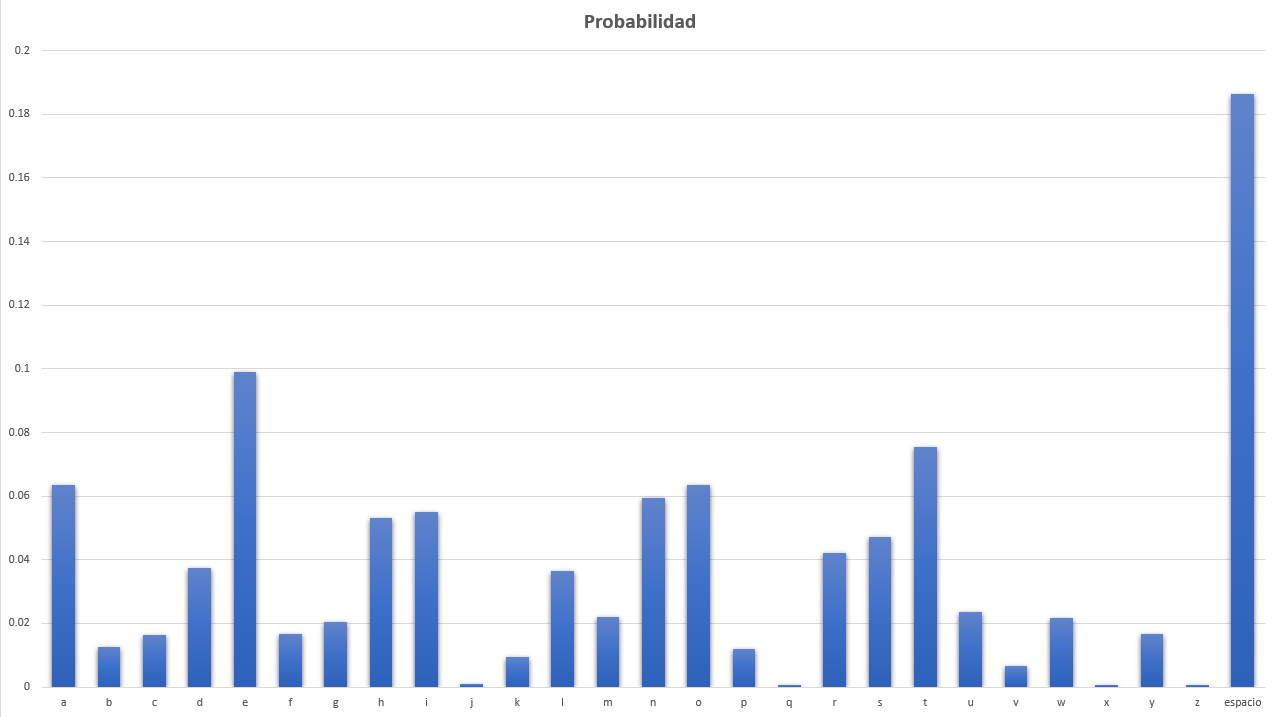
\includegraphics[width=1\textwidth]{ingleSinMemProp.PNG}
    \caption{Logotipo empresa.}
\end{figure}

\end{document}